% !TEX root = ../../UPDATED_main.tex
\subsection*{Publication-scale nucleotide comparisons}

We evaluated fixed GTR+F, GTR+F+G4, and GTR+F+I+G4 models in 1,000 paired replicates per cell, using alignments of 100, 250, or 1,000 sites; focal branch lengths of 4--12; and five-taxon external or 16-taxon internal targets. The merged grid contains 864,000 detail rows and 2,016 summaries, with complete replicate identifiers and no JC-collapse mismatch.

Both GTR+F+G4 formulations lost power as the focal branch length increased, and longer alignments shifted the transition rightward (Fig.~\ref{fig-gtr-g4-power}). Weighting produced its largest shift at 100 sites, where original SatuTe had left the high-power regime but the weighted statistic still detected coherence. Supplementary Figs. S4--S6 report paired differences and the corresponding GTR+F and GTR+F+I+G4 curves.

\begin{figure}[p]
  \centering
  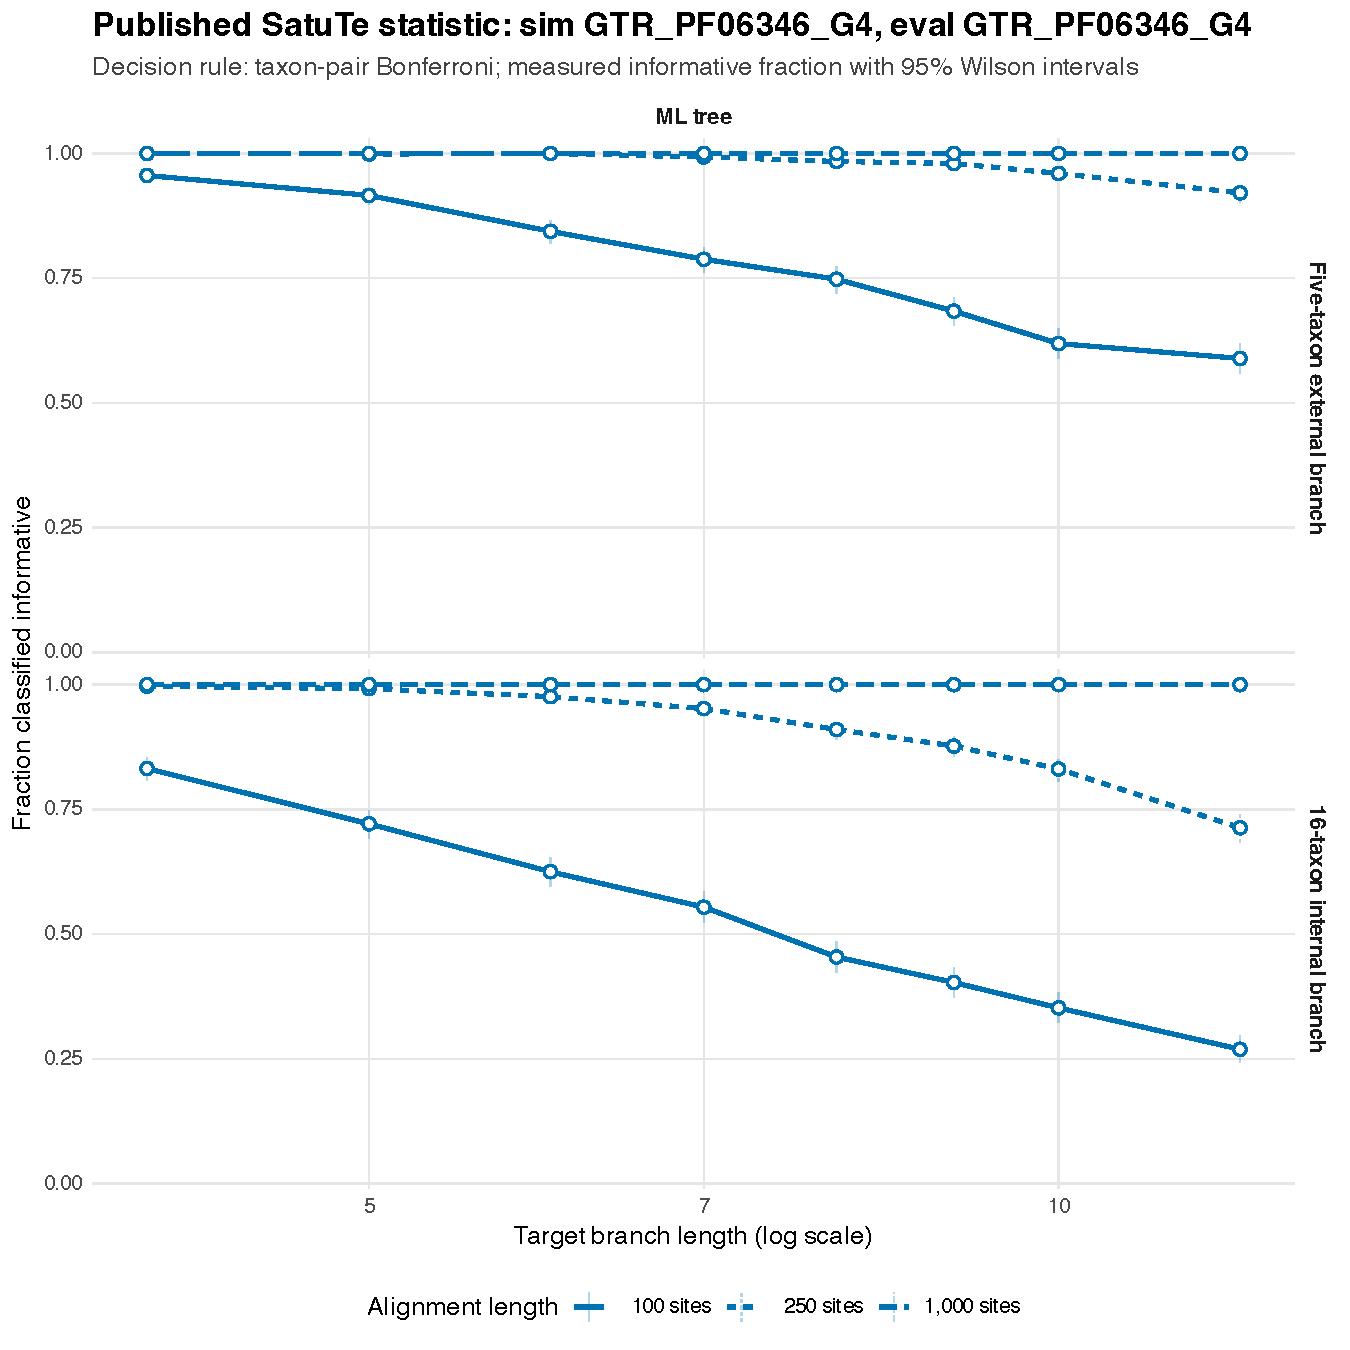
\includegraphics[width=0.49\textwidth]{figures/publication-suite/power/gtr_GTR_PF06346_G4_dominant.pdf}
  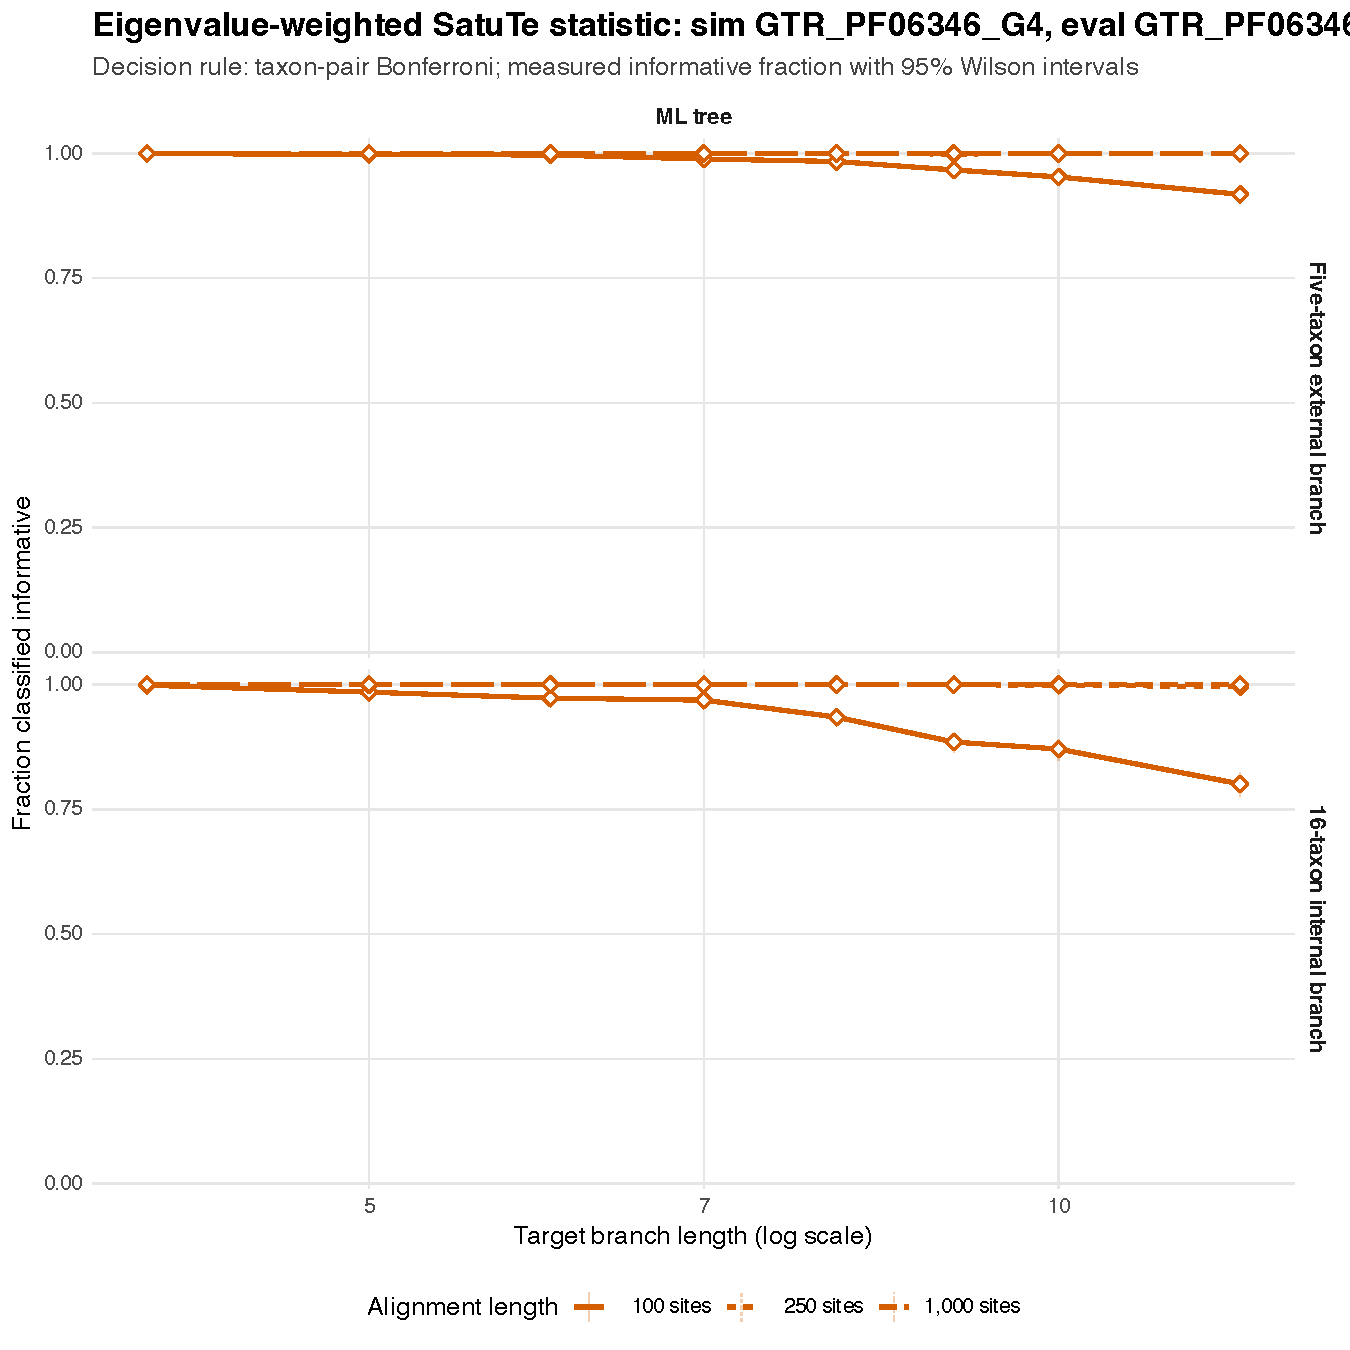
\includegraphics[width=0.49\textwidth]{figures/publication-suite/power/gtr_GTR_PF06346_G4_weighted.pdf}
  \caption{\textbf{Matched GTR+F+G4 power.} \textbf{a,} Original SatuTe statistic. \textbf{b,} Eigenvalue-weighted statistic. Points show informative-call fractions among 1,000 paired replicates under taxon Bonferroni correction; curves are stratified by tree and analysis scenario, and line styles indicate alignment length. Weighting preserves power further into the long-branch regime, particularly at 100 sites.}
  \makeatletter\cref@old@label{fig-gtr-g4-power}\makeatother
\end{figure}

The largest GTR+F+G4 increase was 0.241 without adjustment (95\% bootstrap interval, 0.215--0.269), 0.576 under taxon Bonferroni correction (0.546--0.607), and 0.414 under Benjamini--Yekutieli (BY; 0.384--0.446). All three maxima occurred at 100 sites on the 16-taxon target. The corresponding exact McNemar \(P\) values were \(5.7\times10^{-73}\), \(8.1\times10^{-174}\), and \(4.7\times10^{-125}\).

\subsection*{Model misspecification changes absolute operating characteristics}

We simulated GTR+F alignments and evaluated each alignment under GTR, JC, K2P, or F81. Across 960,000 detail rows, JC and K2P were more liberal than correctly specified GTR, whereas F81, which retains base composition, was substantially closer (Fig.~\ref{fig-gtr-misspec-absolute}). A small paired difference between formulas under a misspecified model therefore does not imply correct absolute calibration.

\begin{figure}[p]
  \centering
  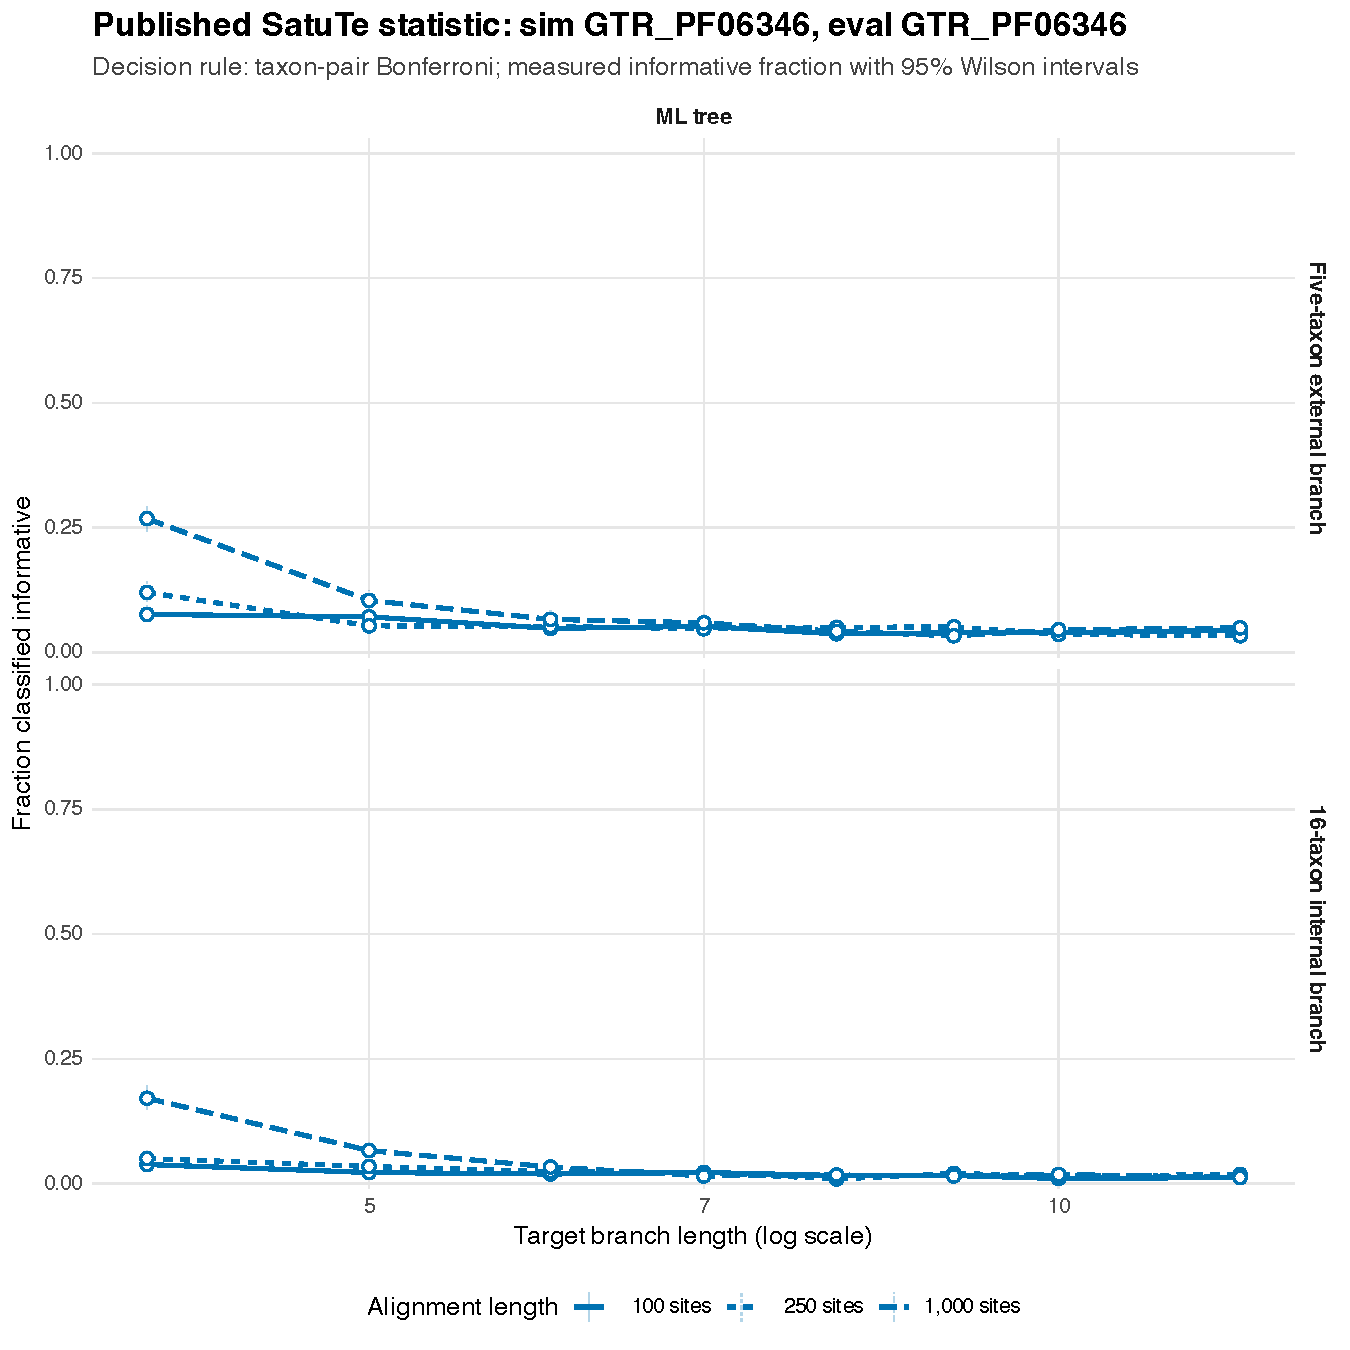
\includegraphics[width=0.49\textwidth]{figures/publication-suite/power/gtr_GTR_PF06346_dominant.pdf}
  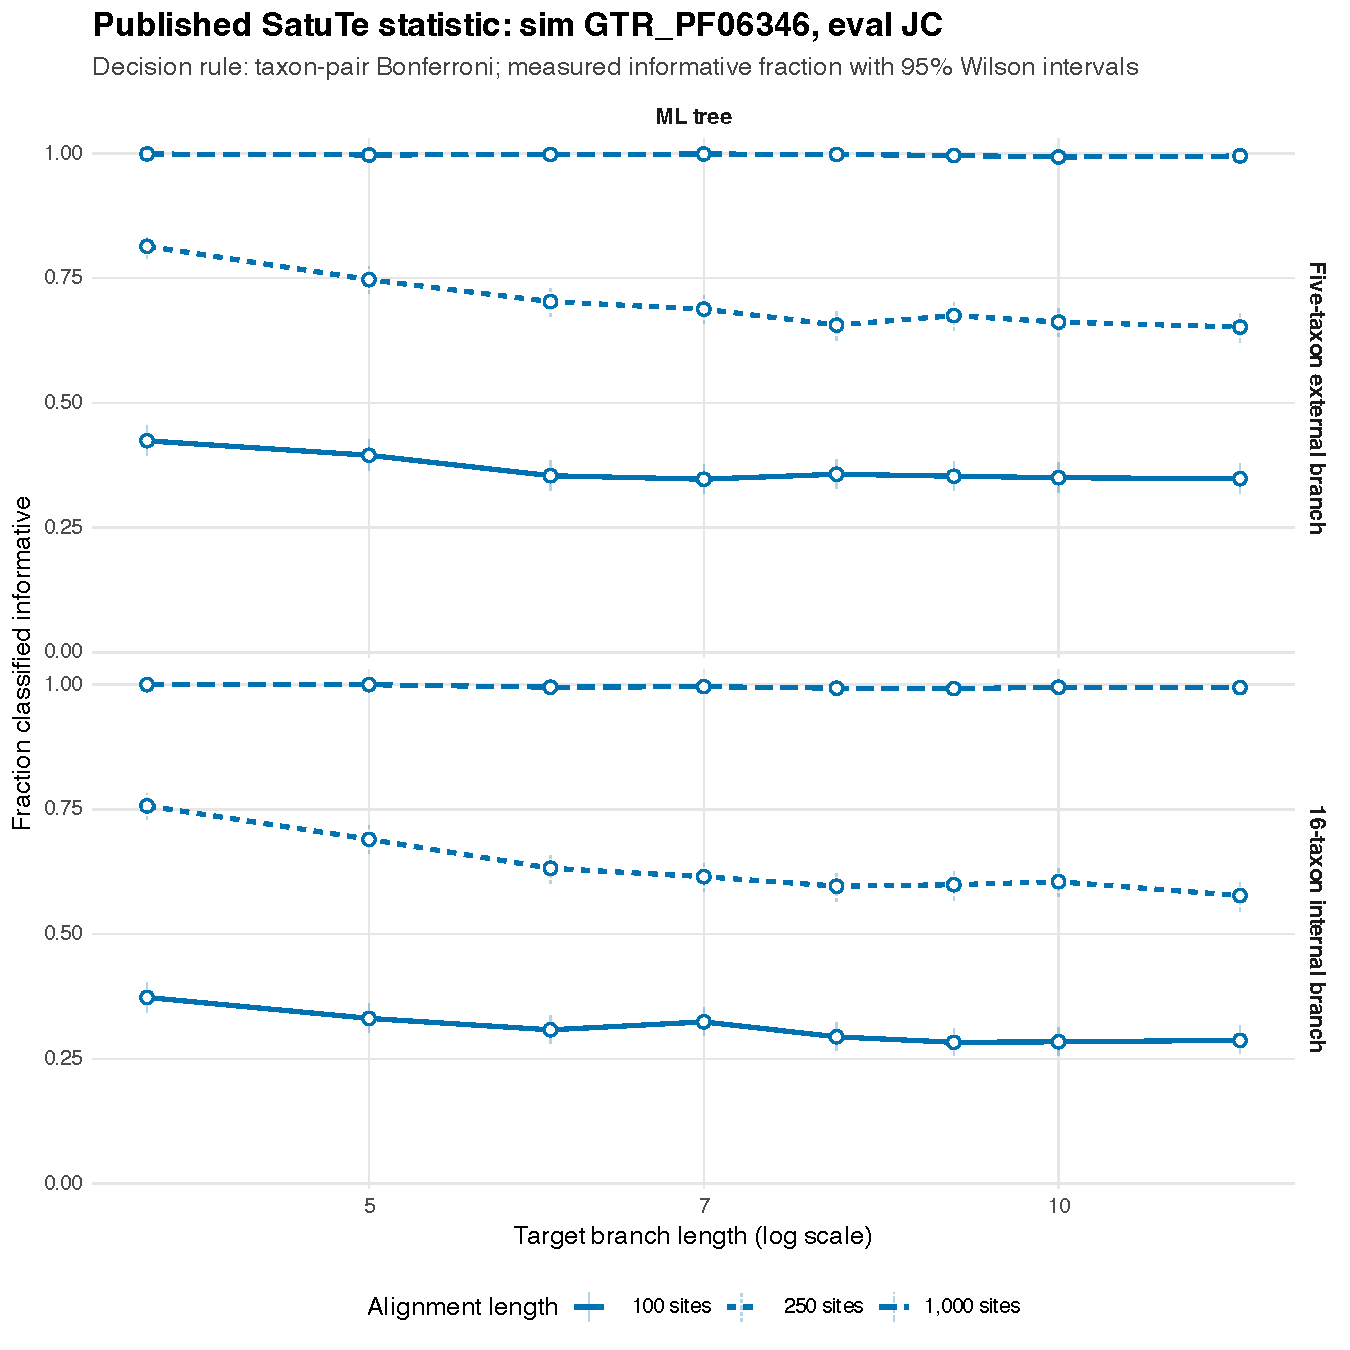
\includegraphics[width=0.49\textwidth]{figures/publication-suite/power/misspec_JC_dominant.pdf}
  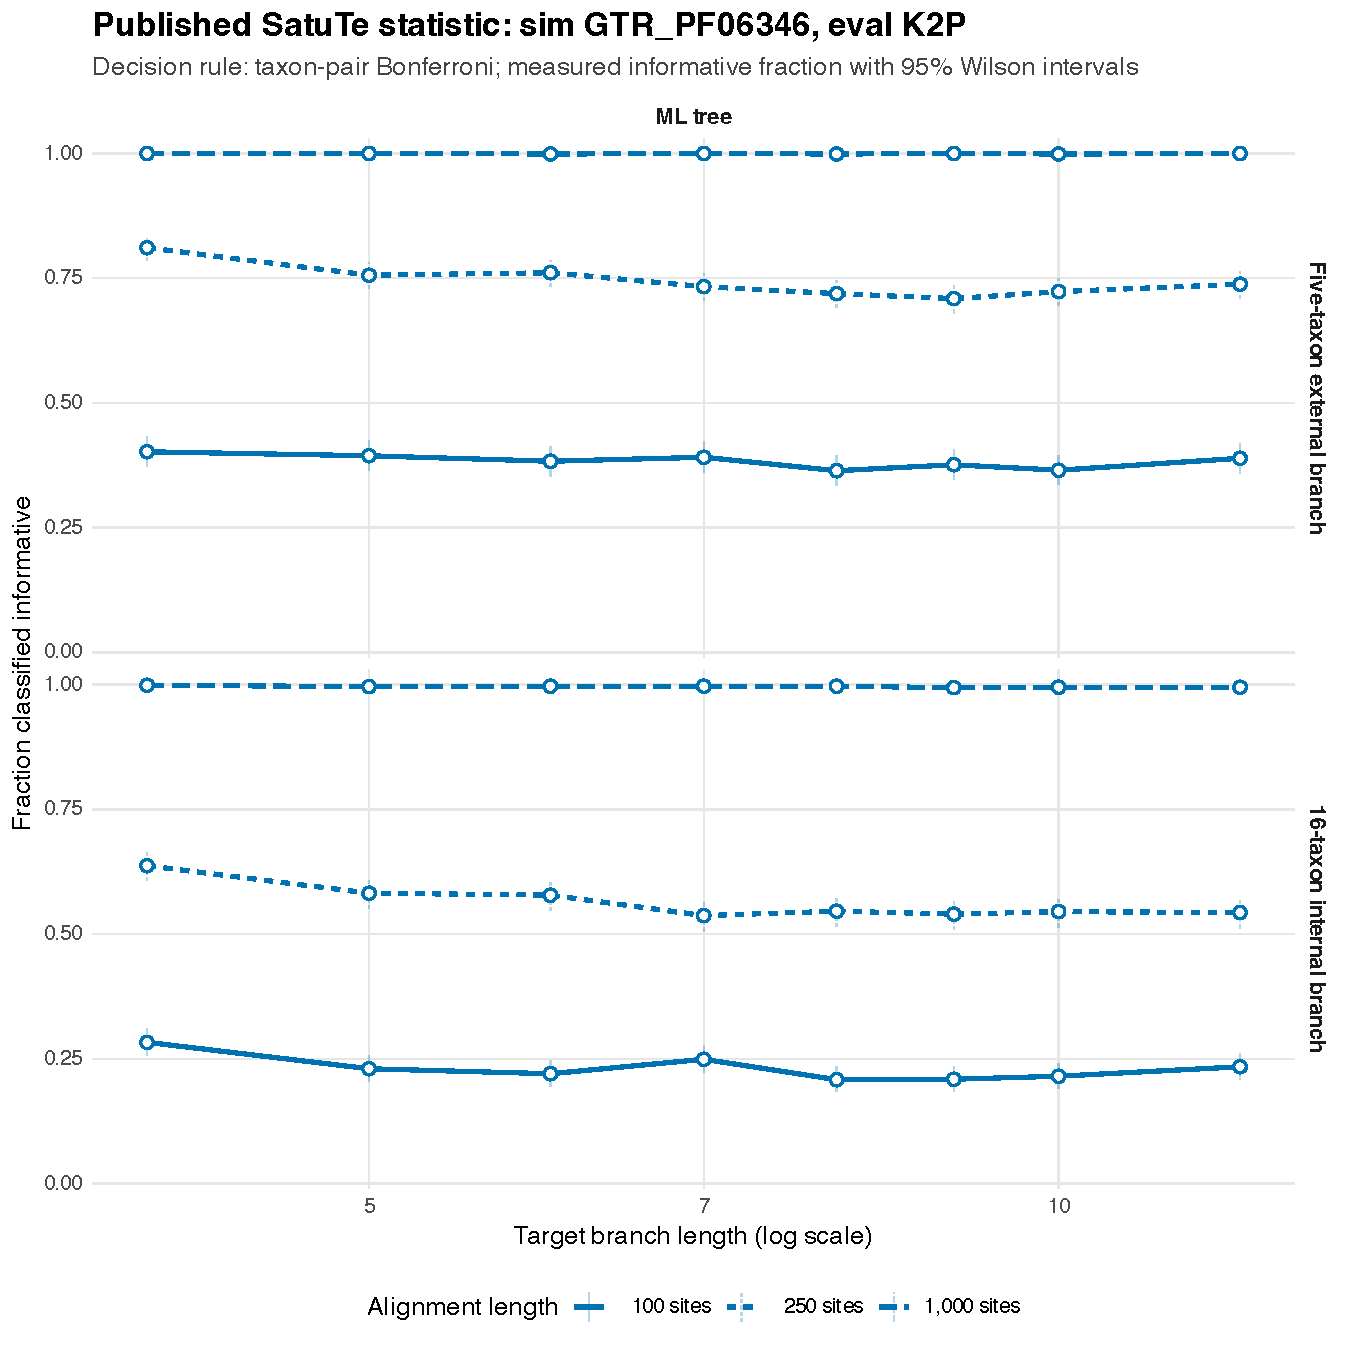
\includegraphics[width=0.49\textwidth]{figures/publication-suite/power/misspec_K2P_dominant.pdf}
  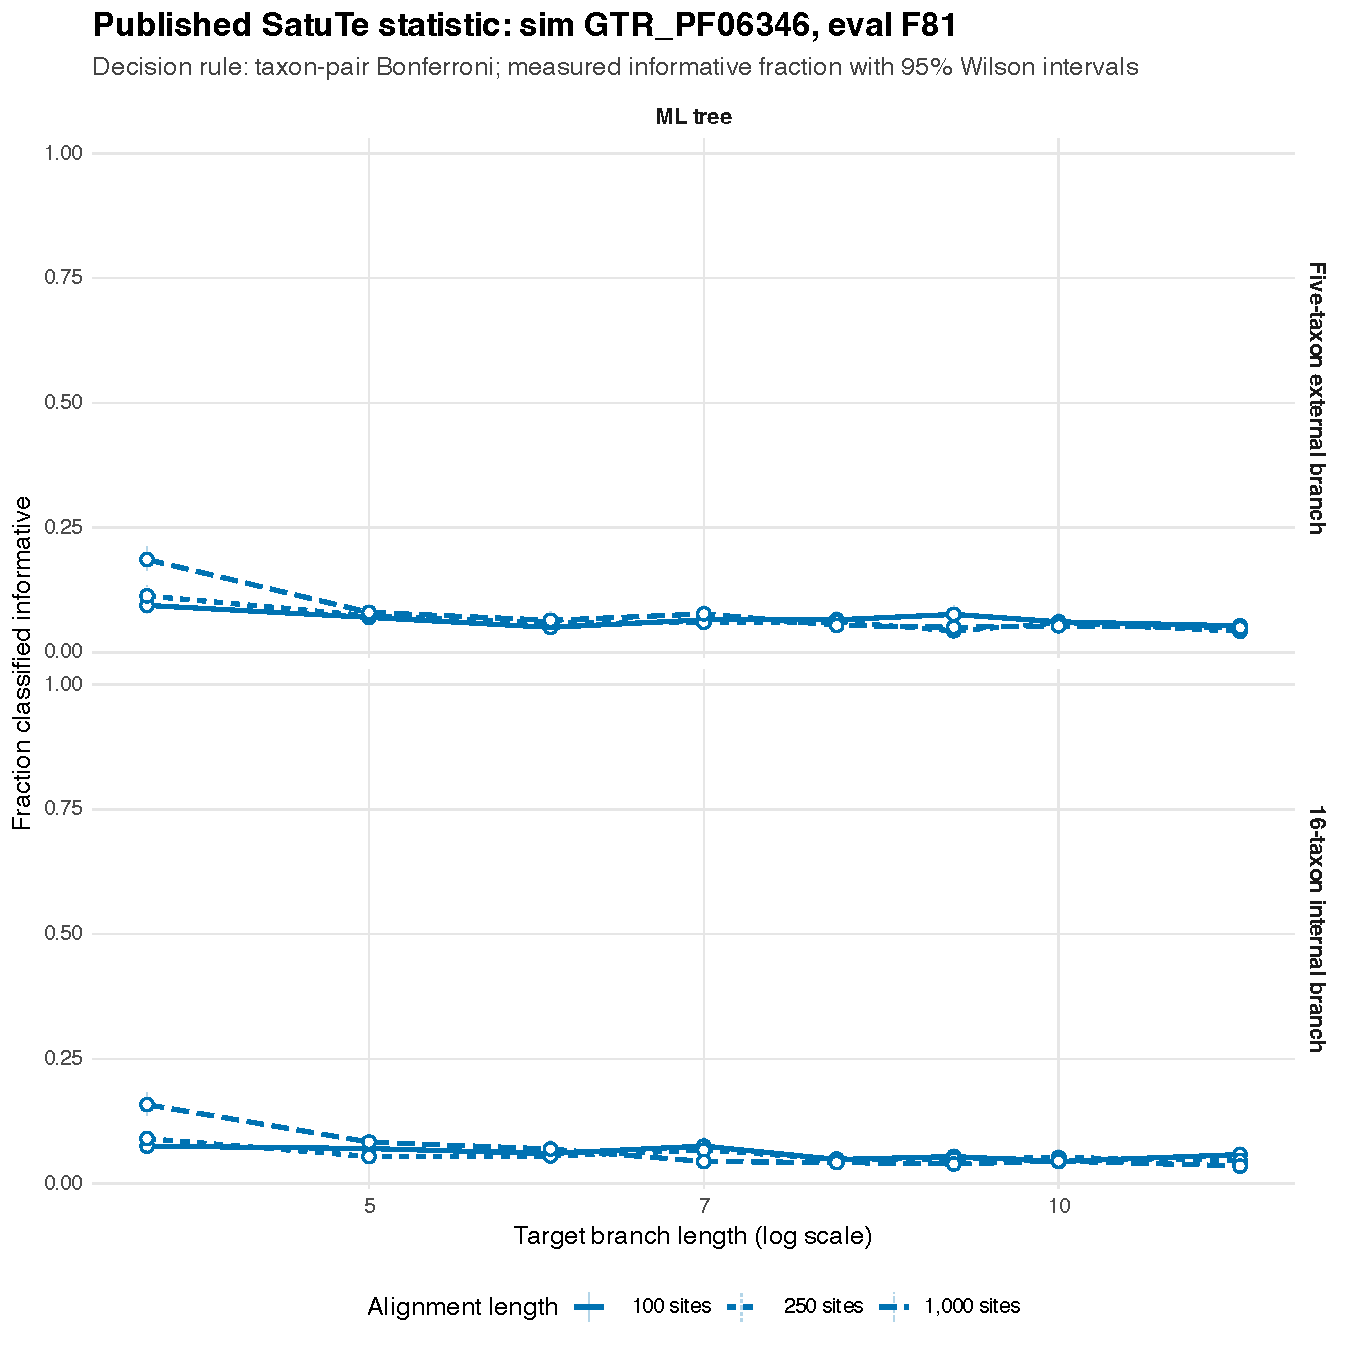
\includegraphics[width=0.49\textwidth]{figures/publication-suite/power/misspec_F81_dominant.pdf}
  \caption{\textbf{Model misspecification changes absolute power.} Original SatuTe taxon-Bonferroni curves for GTR data evaluated under GTR (top left), JC (top right), K2P (bottom left), or F81 (bottom right). JC and K2P are more liberal at long branches, whereas F81 approaches the correctly specified analysis.}
  \makeatletter\cref@old@label{fig-gtr-misspec-absolute}\makeatother
\end{figure}

Within the misspecified analyses, the largest weighted gains were 0.131 without adjustment, 0.206 under taxon Bonferroni correction, and 0.209 under BY. JC remained an exact formula control because its non-stationary eigenvalues are equal. Supplementary Figs. S11--S13 show JC, K2P, and F81 paired differences and weighted curves.

\subsection*{Matched protein power depends strongly on the model}

The matched protein suite used fixed LG+G4, WAG+G4, JTT+G4, and Q.pfam+G4 models. Across 1,728 model--rule--grid cells, weighted-minus-original differences were positive in 831, zero in 897, and negative in none. Maximum taxon-Bonferroni gains were 0.327 for LG, 0.469 for WAG, 0.555 for JTT, and 0.354 for Q.pfam. The complete original, weighted, and paired-difference curves show strong matrix-specific transitions (Supplementary Figs. S7--S10).

\subsection*{Independent truth-labeled calibration supports error control}

Independent calibration used 5,000 exact-null replicates per cell, split equally between threshold training and held-out evaluation, plus 2,000 50:50 mixed-null replicates. In the GTR mixed-null design, power ranged from 0.929 to 0.989 and empirical FDR from zero to 0.00386. Formula-paired differences were at most 0.000571 for power and 0.000143 for FDR, confirming that the larger publication-grid effects are localized to the saturation boundary (Supplementary Fig. S14).

Across 96 cells, held-out rejection ranged from 0.0108 to 0.0644; unadjusted and BY GTR cells ranged from 0.0432 to 0.0596. Sixteen-taxon Bonferroni cells were conservative because only complete tied blocks of discrete adjusted \(P\) values were attainable.
